\documentclass{article}
\usepackage{microtype}
\usepackage{graphicx}
\usepackage{subfigure}
\usepackage{subcaption}
\usepackage{booktabs}
\usepackage[style=authoryear,backend=biber]{biblatex}
\addbibresource{References.bib}
\usepackage{amsmath}
\usepackage{amsfonts}
\usepackage{amsthm}
\usepackage{physics}
\usepackage{fancyvrb}
\usepackage{listings}
\usepackage{xcolor}
\usepackage{caption}
\usepackage{xurl}
\usepackage{url}
\usepackage{hyperref}
\newcommand{\theHalgorithm}{\arabic{algorithm}}
\usepackage{accessibility}
\usepackage{Coursework}

\begin{document}
\cwtitle{COMP1680 - Clouds, Grids and Virtualisation Coursework Report}
\begin{cwauthorlist}
\cwauthor{Azhar Muhammed - 001364857}
\cwauthor{Word Count: }
\end{cwauthorlist}

\section{Parallel Processing using Cloud Computing}

In the contemporary landscape of computational technologies, small consultancy firms face critical decisions regarding their computational infrastructure. The choice between adopting cloud computing services or investing in an onsite High-Performance Computing (HPC) system significantly impacts operational efficiency, scalability, and financial expenditure. This report evaluates these options for a consultancy company comprising 30 consultants utilizing approximately 1,400 CPU hours each month. The analysis focuses on the advantages and disadvantages of leading cloud service providers---Amazon Web Services (AWS), Microsoft Azure, and Google Cloud Platform (GCP)---compared to an onsite HPC system for multicore workloads using batch processing. A comprehensive financial cost comparison is provided, culminating in a recommendation that aligns with the company's strategic objectives.

\subsection{Analysis of Cloud Providers vs. Onsite HPC for Multicore Workloads}

Cloud computing has revolutionized the way businesses handle computational workloads, offering scalable resources and flexible pricing models. In contrast, onsite HPC systems provide dedicated resources but require substantial initial investments and ongoing maintenance.

\begin{table}[H]
    \centering
    \caption{Onsite HPC Costs Breakdown}
    \label{tab:hpc_costs}
    \begin{tabular}{lrr}
    \toprule
    \textbf{Cost Item} & \textbf{Minimum (\$)} & \textbf{Maximum (\$)} \\
    \midrule
    \textbf{Initial Setup Costs} & & \\
    \quad HPC Hardware & 80,000 & 120,000 \\
    \quad Cooling Systems & 10,000 & 20,000 \\
    \quad Power Supplies and UPS & 5,000 & 10,000 \\
    \quad Networking Equipment & 5,000 & 10,000 \\
    \textbf{Total Initial Setup Cost} & \textbf{100,000} & \textbf{160,000} \\
    \midrule
    \textbf{Annual Operating Costs} & & \\
    \quad Maintenance and Support Contracts & 10,000 & 15,000 \\
    \quad Energy Consumption & 756 & 756 \\
    \quad IT Personnel Salary & 50,000 & 70,000 \\
    \textbf{Total Annual Operating Costs} & \textbf{60,756} & \textbf{85,756} \\
    \midrule
    \textbf{Hardware Upgrade Costs (Every 4--5 Years)} & 50,000 & 112,000 \\
    \midrule
    \textbf{Total 5-Year Cost} & \textbf{453,780} & \textbf{700,780} \\
    \bottomrule
    \end{tabular}
    \end{table}

\subsubsection{Advantages of Cloud Computing Over Onsite HPC}

Cloud computing offers several advantages over onsite HPC systems, particularly for small consultancies:
\begin{itemize}
    \item \textbf{Scalability and Flexibility:} Cloud services allow dynamic scaling of computational resources to match workload demands. This elasticity is essential for batch processing tasks that may have variable computational needs \parencite{armbrust2010cloud}.
    \item \textbf{Cost Efficiency:} With pay-as-you-go models, companies avoid the substantial upfront capital expenditure associated with purchasing HPC hardware. Operational costs are aligned with actual usage, enhancing financial predictability \parencite{li2019decision}.
    \item \textbf{Maintenance and Operational Overhead:} Cloud providers handle hardware maintenance, software updates, and security patches, reducing the burden on internal IT staff \parencite{marinescu2013cloud}.
    \item \textbf{Access to Advanced Technologies:} Cloud platforms frequently update their offerings, providing access to the latest hardware and software innovations without additional costs \parencite{dillon2010cloud}.
\end{itemize}

\subsubsection{Disadvantages of Cloud Computing}

Despite these advantages, cloud computing presents certain challenges:
\begin{itemize}
    \item \textbf{Data Security and Compliance:} Relying on third-party providers raises concerns about data sovereignty and compliance with regulations such as GDPR \parencite{hashem2015bigdata}.
    \item \textbf{Performance Variability:} Multi-tenant cloud environments can lead to inconsistent performance due to resource contention \parencite{leitner2016patterns}.
    \item \textbf{Potential for Unexpected Costs:} Without proper management, costs can escalate due to factors like data egress fees and underutilized resources \parencite{rehman2018cloud}.
\end{itemize}

\subsection{Comparison of Leading Cloud Providers}

\textbf{Amazon Web Services (AWS):}
AWS offers a broad range of services suitable for batch processing, such as AWS Batch and EC2 compute-optimized instances. It provides robust scalability and a variety of pricing models, including on-demand, reserved, and spot instances \parencite{awspricing}. AWS's global infrastructure ensures high availability and low latency.

\textbf{Microsoft Azure:}
Azure provides services like Azure Batch and compute-optimized virtual machines suitable for parallel processing tasks. It integrates seamlessly with other Microsoft products, which can be advantageous for companies already utilizing Microsoft ecosystems \parencite{azurepricing}. Azure offers competitive pricing and various discount options, such as reserved instances.

\textbf{Google Cloud Platform (GCP):}
GCP's Compute Engine and preemptible virtual machines offer cost-effective solutions for batch processing workloads. GCP emphasizes sustained use discounts, automatically reducing costs for consistent usage without long-term commitments \parencite{gcppricing}. Google's expertise in containerization and Kubernetes can benefit firms looking to adopt modern deployment practices.

\begin{table}[H]
    \centering
    \caption{Cloud Computing Costs for AWS, Azure, and GCP}
    \label{tab:cloud_costs}
    \begin{tabular}{lccc}
    \toprule
    \textbf{Cost Item} & \textbf{AWS} & \textbf{Azure} & \textbf{GCP} \\
    \midrule
    \textbf{Instance Type} & c6a.large & F2s\_v2 & n2-standard-2 \\
    \textbf{vCPUs} & 2 & 2 & 2 \\
    \textbf{Price per Hour (\$)} & 0.085 & 0.085 & 0.084 \\
    \textbf{Monthly Compute Cost (\$)} & 119.00 & 119.00 & 117.60 \\
    \textbf{Storage Cost per Month (\$)} & 20.00 & 20.00 & 20.00 \\
    \textbf{Data Transfer Cost per Month (\$)} & 10.00 & 10.00 & 10.00 \\
    \textbf{Total Monthly Cost (\$)} & 149.00 & 149.00 & 147.60 \\
    \textbf{Annual Cost (\$)} & 1,788.00 & 1,788.00 & 1,771.20 \\
    \textbf{5-Year Cost (\$)} & 8,940.00 & 8,940.00 & 8,856.00 \\
    \bottomrule
    \end{tabular}
    \end{table}

\subsubsection{Comparison Between Cloud Providers}
While all three providers offer similar core services, differences exist in pricing models, discount structures, and additional services:
\begin{itemize}
    \item \textbf{Pricing Models:} AWS and Azure offer reserved instances for long-term commitments, while GCP provides sustained use discounts without upfront commitments.
    \item \textbf{Ecosystem Integration:} Azure may be preferable for companies using Microsoft tools, whereas AWS has a more extensive range of services and a mature ecosystem.
    \item \textbf{Specialized Services:} GCP excels in machine learning and big data analytics services, which could be beneficial depending on the consultancy's focus.
\end{itemize}

\subsubsection{Advantages of Onsite HPC}
Onsite HPC systems offer complete control over hardware and software configurations. They may provide performance benefits due to dedicated resources and reduced latency \parencite{stergiou2018iot}. Additionally, data remains on-premises, which can alleviate certain security and compliance concerns.

\subsubsection{Disadvantages of Onsite HPC}

The primary drawbacks of onsite HPC include:

\begin{itemize}
    \item \textbf{High Initial Capital Expenditure:} Significant upfront investment is required for hardware, infrastructure, and installation.
    \item \textbf{Maintenance Costs:} Ongoing costs for maintenance, energy consumption, and staffing can be substantial.
    \item \textbf{Lack of Scalability:} Scaling up requires additional hardware purchases, leading to potential underutilization during periods of low demand.
\end{itemize}

\subsubsection{Financial Cost Comparison}
A detailed financial analysis over a five-year period highlights the cost implications of both options.

\begin{table}[H]
    \centering
    \caption{Five-Year Total Cost Comparison}
    \label{tab:total_cost_comparison}
    \begin{tabular}{lrr}
    \toprule
    \textbf{Option} & \textbf{Minimum Total Cost (\$)} & \textbf{Maximum Total Cost (\$)} \\
    \midrule
    Onsite HPC & 453,780 & 700,780 \\
    Cloud Computing (AWS) & 8,940 & 8,940 \\
    Cloud Computing (Azure) & 8,940 & 8,940 \\
    Cloud Computing (GCP) & 8,856 & 8,856 \\
    \midrule
    \textbf{Cost Savings with Cloud Computing} & \textbf{444,924} & \textbf{691,924} \\
    \bottomrule
    \end{tabular}
    \end{table}


\subsubsection{Onsite HPC Costs}
\textbf{Initial Setup Costs:}
The purchase of HPC hardware, including high-performance servers, networking equipment, and storage systems, is estimated between \$80,000 and \$120,000. Infrastructure costs, encompassing cooling systems, power supplies, and additional networking equipment, add another \$20,000 to \$40,000. Thus, the total initial setup cost ranges from \$100,000 to \$160,000.

\textbf{Annual Operating Costs:}
Maintenance and support contracts cost between \$10,000 and \$15,000 annually. Energy consumption is calculated based on an estimated 0.3 kWh per CPU hour at \$0.15 per kWh, resulting in an annual energy cost of \$756. Staffing requires a part-time HPC specialist, with salary expenses ranging from \$50,000 to \$70,000 per year. The total annual operating costs amount to \$60,756 to \$85,756.

\textbf{Hardware Upgrade Costs:}
Upgrades are anticipated every 4-5 years, costing 50-70\% of the initial hardware investment, equating to \$50,000 to \$112,000.

\textbf{Total Five-Year Cost:}
Combining the initial setup, operating costs over five years, and hardware upgrades, the total expenditure ranges from \$453,780 to \$700,780.

\subsubsection{Cloud Computing Costs}
\textbf{Amazon Web Services (AWS):}
To fulfill the requirement of 1,400 CPU hours per month, AWS offers the c6a.large instance at \$0.085 per hour. The monthly compute cost is \$119, with additional storage and data transfer costs estimated at \$30 per month. The total monthly cost is \$149, leading to an annual cost of \$1,788 and a five-year cost of \$8,940. Potential discounts through reserved instances or spot instances can further reduce expenses.

\textbf{Microsoft Azure:}
Azure's F2s\_v2 instance, also priced at approximately \$0.085 per hour, results in identical compute costs to AWS. Including storage and data transfer, the total monthly cost is \$149, with a five-year cost of \$8,940.

\textbf{Google Cloud Platform (GCP):}
GCP's n2-standard-2 instance costs \$0.084 per hour, leading to a monthly compute cost of \$117.60. Including storage and data transfer, the total monthly cost is \$147.60. The annual cost is \$1,771.20, and the five-year cost is \$8,856. Sustained use discounts may reduce costs by up to 30\%.

\subsubsection{Total Cost Comparison}
Over five years, the total cost for cloud computing ranges from \$8,856 to \$8,940, significantly lower than the onsite HPC cost of \$453,780 to \$700,780. The cost savings with cloud computing amount to \$444,924 to \$691,924 over five years.

\subsection{Recommendation}

Based on the analysis of operational and financial factors, it is recommended that the consultancy company adopts a cloud computing solution for its parallel processing needs.

\textbf{Significant Cost Savings:} The financial comparison demonstrates substantial cost savings with cloud computing, reducing expenditures by over \$440,000 over five years. This capital can be allocated to other strategic initiatives within the company.

\textbf{Operational Efficiency:} Cloud computing minimizes the need for in-house IT maintenance, allowing consultants to focus on core business activities. The responsibility for hardware maintenance and updates lies with the cloud provider, enhancing operational efficiency.

\textbf{Flexibility and Scalability:} Cloud services offer unparalleled flexibility, with the ability to adjust resources to match workload demands seamlessly. This scalability supports business growth without the need for additional infrastructure investment.

\textbf{Risk Mitigation:} Cloud computing eliminates risks associated with hardware failures and obsolescence. Providers offer high availability and disaster recovery solutions, ensuring business continuity.

\subsubsection{Platform Selection}
While all three major cloud providers offer services that meet the company's needs, slight distinctions may influence the decision:
\begin{itemize}
    \item \textbf{AWS:} With its extensive range of services and mature ecosystem, AWS is suitable for companies seeking a broad array of tools and global infrastructure.
    \item \textbf{Azure:} For firms already utilizing Microsoft products, Azure offers seamless integration and may provide operational efficiencies.
    \item \textbf{GCP:} Companies interested in advanced analytics and machine learning capabilities may prefer GCP due to its strengths in these areas.
\end{itemize}
Given the consultancy's size and requirements, any of these providers could be appropriate. A detailed assessment of existing partnerships, staff expertise, and specific service offerings should guide the final selection. the final selection. The consultancy should also consider any existing vendor relationships or preferred ecosystems when making the final decision.

\subsubsection{Implementation Considerations}
To maximize the benefits of cloud computing, the company should take the following steps during the implementation phase:

\begin{itemize}
    \item \textbf{Leverage Cost Savings Opportunities:} Utilize reserved instances or savings plans for predictable workloads and explore spot instances for non-critical tasks to reduce costs.
    \item \textbf{Implement Cost Management Practices:} Use cloud monitoring tools to track resource utilization, set alerts for unexpected cost spikes, and establish budgets to manage cloud spending effectively.
    \item \textbf{Ensure Security and Compliance:} Establish robust cloud security policies, implement encryption for sensitive data, and leverage the cloud provider's compliance certifications to meet regulatory requirements.
    \item \textbf{Provide Staff Training:} Equip consultants with the necessary skills to use cloud services effectively, ensuring a smooth transition and minimizing resistance to the new system.
\end{itemize}

\begin{table}[H]
    \centering
    \caption{Comparison of Cloud Computing and Onsite HPC}
    \label{tab:advantages_disadvantages}
    \begin{tabular}{p{5cm}p{5cm}p{5cm}}
    \toprule
    \textbf{Criteria} & \textbf{Cloud Computing} & \textbf{Onsite HPC} \\
    \midrule
    \textbf{Scalability and Flexibility} & High; resources can be scaled up or down easily & Limited; scaling requires hardware investment \\
    \textbf{Initial Capital Expenditure} & Low; pay-as-you-go model & High; significant upfront costs \\
    \textbf{Maintenance Overhead} & Low; provider handles maintenance & High; requires dedicated IT staff \\
    \textbf{Risk of Obsolescence} & Low; access to latest technology & High; hardware can become outdated \\
    \textbf{Energy Consumption} & Lower; optimized data centers & Higher; increased operational costs \\
    \textbf{Data Control} & Less control; data stored off-premises & Full control; data stored on-site \\
    \textbf{Security and Compliance} & High; robust security measures and certifications & Dependent on in-house capabilities \\
    \textbf{Total Cost over 5 Years} & \$8,856 -- \$8,940 & \$453,780 -- \$700,780 \\
    \bottomrule
    \end{tabular}
    \end{table}

\subsubsection{Conclusion}
Transitioning to cloud computing is a strategic decision that aligns with the consultancy company's operational needs and financial objectives. The substantial cost savings, coupled with enhanced scalability and reduced maintenance burdens, make cloud services the optimal choice over an onsite HPC system. By adopting cloud computing, the company positions itself to leverage advanced technologies, respond agilely to market demands, and focus its resources on delivering value to clients.

\section{Parallel Programming Exercise}

\subsection{Step 1}

The C program was adapted to simulate the temperature distribution in a rectangular 2D grid with specific boundary conditions: the top boundary at 15°C, the bottom at 60°C, the left at 47°C, and the right at 100°C. These conditions were implemented by setting the corresponding edges of the grid to the specified temperatures.

In the code, after initializing the entire grid to an initial temperature (e.g., 30°C), the boundary conditions are applied:

\begin{lstlisting}[style=CStyle, caption={Setting Boundary Conditions}]
// Set boundary conditions
for (int i = 1; i <= m; i++) {
    t[i][0] = LEFT_TEMP;      // Left boundary set to 47°C
    t[i][n + 1] = RIGHT_TEMP; // Right boundary set to 100°C
}
for (int j = 1; j <= n; j++) {
    t[0][j] = TOP_TEMP;        // Top boundary set to 15°C
    t[m + 1][j] = BOTTOM_TEMP; // Bottom boundary set to 60°C
}

// Set corner temperatures as average of adjacent boundaries
t[0][0] = (TOP_TEMP + LEFT_TEMP) / 2.0;             // Top-left corner
t[0][n + 1] = (TOP_TEMP + RIGHT_TEMP) / 2.0;        // Top-right corner
t[m + 1][0] = (BOTTOM_TEMP + LEFT_TEMP) / 2.0;      // Bottom-left corner
t[m + 1][n + 1] = (BOTTOM_TEMP + RIGHT_TEMP) / 2.0; // Bottom-right corner
\end{lstlisting}

These code snippets ensure that the boundary temperatures are correctly set according to the problem's specifications. The corners are handled separately by averaging the temperatures of the adjacent boundaries to avoid anomalies at those points.

\subsubsection{Execution Time}

To measure the execution time of the program, the \texttt{time.h} library is included, and timing functions are used:

\begin{lstlisting}[style=CStyle, caption={Execution Time Measurement}]
#include <time.h> // For measuring execution time

// Start timing the execution
clock_t start = clock();

// ... [Jacobi iteration loop] ...

// Calculate execution time
clock_t end = clock();
double cpu_time_used = ((double)(end - start)) / CLOCKS_PER_SEC;

// Print results
printf("Execution time: %f seconds\n", cpu_time_used);
\end{lstlisting}

The \texttt{clock()} function records the processor time consumed by the program. By capturing the time before and after the main computation loop and calculating the difference, the execution time is obtained. This measurement is crucial for comparing performance across different grid sizes and compiler optimization levels.

\subsubsection{Adjustments for Realistic Execution Time Measurements}

To obtain accurate execution time measurements, it is important to prevent the program from printing large amounts of data, which can significantly affect performance. In the code, the grid values are only printed if the grid size is small (e.g., 10x10 or smaller):

\begin{lstlisting}[style=CStyle, caption={Printing Grid Values for Small Grids}]
// Print grid values for small grids (10x10 or smaller)
if (m <= 10 && n <= 10) {
    for (int i = 0; i <= m + 1; i++) {
        for (int j = 0; j <= n + 1; j++) {
            printf("%3.5lf ", t[i][j]);
        }
        printf("\n");
    }
}
\end{lstlisting}

By restricting the output for larger grids, the program avoids the overhead associated with I/O operations, leading to more accurate timing of the computational aspects.

\subsubsection{Automation of Testing with Bash Script}

The provided Bash script automates the compilation and execution of the program across different optimization levels (\texttt{-O0} to \texttt{-O3}) and grid sizes (150x150, 200x200, 250x250). The script performs the following tasks:

1. \textbf{Compiler Selection:}

   The script checks for the availability of \texttt{gcc-14}; if not found, it defaults to \texttt{gcc}:

   \begin{lstlisting}[style=CStyle, caption={Setting Boundary Conditions}]
   if command -v gcc-14 &> /dev/null; then
       COMPILER=gcc-14
   else
       COMPILER=gcc
   fi
   \end{lstlisting}

2. \textbf{Compilation with Different Optimization Levels:}

   The program is compiled multiple times with different optimization flags:

   \begin{lstlisting}[style=CStyle, caption={Setting Boundary Conditions}]
   for optmlvl in 0 1 2 3; do
       $COMPILER -std=c99 -O${optmlvl} jacobi2d-Step1.c -o jacobi2d-Step1-O${optmlvl}
       # Error checking omitted for brevity
   done
   \end{lstlisting}

3. \textbf{Execution Across Grid Sizes and Optimization Levels:}

   The script runs the compiled programs for each combination of grid size and optimization level, capturing the output:

   \begin{lstlisting}[style=CStyle, caption={Setting Boundary Conditions}]
   for size in 150 200 250; do
       for optmlvl in 0 1 2 3; do
           echo "Testing grid size of ${size}x${size} with optimization level -O${optmlvl}" >> jacobi2d-Step1.txt
           ./jacobi2d-Step1-O${optmlvl} $size $size 0.000100 >> jacobi2d-Step1.txt
           echo "--------------------------------------" >> jacobi2d-Step1.txt
       done
   done
    \end{lstlisting}

This automated approach ensures consistency and efficiency in data collection, facilitating the analysis of how different optimization levels impact execution time for various grid sizes.

\subsubsection{Results and Observations}

The output collected demonstrates how compiler optimization levels affect the program's performance. Generally, higher optimization levels \texttt{-O1}, \texttt{-O2}, \texttt{-O3}) result in reduced execution times compared to no optimization (\texttt{-O0}). The data also shows that as the grid size increases, the execution time increases, which is expected due to the larger computational workload.

\subsubsection{Considerations Regarding Compiler Optimizations}

It is noted that aggressive compiler optimizations can potentially alter the program's behavior. In this case, the program was tested across all optimization levels without any observed issues. However, caution is advised, and validation checks should be included to ensure that the optimizations do not introduce unintended side effects.

\begin{table}[H]
    \centering
    \caption{Execution Times for Different Grid Sizes and Optimization Levels}
    \label{tab:execution_times}
    \begin{tabular}{lrrcccc}
    \toprule
    \textbf{Grid Size} & \textbf{Iterations} & \textbf{Maximum Difference ($difmax$)} & \textbf{-O0 (s)} & \textbf{-O1 (s)} & \textbf{-O2 (s)} & \textbf{-O3 (s)} \\
    \midrule
    150x150 & 20,763 & $9.9990 \times 10^{-5}$ & 2.492 & 0.468 & 0.443 & 0.413 \\
    200x200 & 32,108 & $9.9992 \times 10^{-5}$ & 6.879 & 1.254 & 1.150 & 1.062 \\
    250x250 & 44,398 & $9.9994 \times 10^{-5}$ & 14.678 & 2.697 & 2.489 & 2.361 \\
    \bottomrule
    \end{tabular}
\end{table}

\subsubsection{Conclusion}

The modifications to the program successfully implemented the specified boundary conditions and enabled the measurement of execution time. The use of a Bash script to automate testing across different grid sizes and optimization levels provided valuable insights into the program's performance characteristics. These results form a solid foundation for further analysis and optimization in subsequent steps of the coursework.

\subsection{Step 2}

The Jacobi 2D grid problem was extended from its sequential implementation to a parallel version using OpenMP. The primary objective was to modify the existing code to incorporate OpenMP directives for parallel execution, compile it with OpenMP support, and test its correctness using multiple threads. The performance was compared across different thread counts to observe the scalability and correctness of the parallel implementation.

\subsubsection{Code Modifications for Parallel Execution}

The original sequential code was adapted to leverage OpenMP for parallel processing. Key modifications were made to parallelize the computation-intensive sections while ensuring thread safety and correctness.

1. \textbf{Including OpenMP Header}

   The OpenMP library was included by adding the header file:

   \begin{lstlisting}[style=CStyle, caption={OpenMP Header Inclusion}]
   #include <omp.h>
   \end{lstlisting}

2. \textbf{Parallel Initialization}

    The initialization of the temperature grids was parallelized using OpenMP directives \parencite{chapman2007openmp}. The \texttt{\#pragma omp parallel} directive was used to define a parallel region, and loops were parallelized using \texttt{\#pragma omp for} with appropriate scheduling:

   \begin{lstlisting}[style=CStyle, caption={Parallel Initialization}]
   #pragma omp parallel
   {
       // Initialize interior points to 30.0
       #pragma omp for collapse(2) schedule(static) nowait
       for (i = 0; i <= m + 1; i++) {
           for (j = 0; j <= n + 1; j++) {
               t[i][j] = 30.0;
               tnew[i][j] = 30.0;
           }
       }

       // Set boundary temperatures
       #pragma omp for schedule(static) nowait
       for (i = 1; i <= m; i++) {
           t[i][0] = LEFT_TEMP;
           t[i][n + 1] = RIGHT_TEMP;
       }

       #pragma omp for schedule(static)
       for (j = 1; j <= n; j++) {
           t[0][j] = TOP_TEMP;
           t[m + 1][j] = BOTTOM_TEMP;
       }
   }
   \end{lstlisting}

    \begin{itemize}
        \item \textbf{Use of \texttt{collapse(2)}:} This clause was used to collapse the two nested loops into a single loop for parallel execution \parencite{openmp}, enhancing load balancing among threads.
        \item \textbf{Scheduling and \texttt{nowait}:} Static scheduling was chosen for simplicity, and the \texttt{nowait} clause was used to eliminate unnecessary barriers, improving performance.
    \end{itemize}

3. \textbf{Parallel Main Iteration Loop:}

   The main computation loop, which performs the Jacobi iteration, was parallelized:

   \begin{lstlisting}[style=CStyle, caption={Parallel Main Iteration Loop}]
   while (difmax > tol) {
       iter++;
       difmax = 0.0;

       #pragma omp parallel
       {
           // Compute new temperature values
           #pragma omp for private(j) schedule(static) nowait
           for (i = 1; i <= m; i++) {
               for (j = 1; j <= n; j++) {
                   tnew[i][j] = (t[i-1][j] + t[i+1][j] + t[i][j-1] + t[i][j+1]) / 4.0;
               }
           }

           // Update temperatures and compute maximum difference
           #pragma omp for private(j, diff) reduction(max:difmax)
           for (i = 1; i <= m; i++) {
               for (j = 1; j <= n; j++) {
                   diff = fabs(tnew[i][j] - t[i][j]);
                   difmax = (diff > difmax) ? diff : difmax;
                   t[i][j] = tnew[i][j];
               }
           }
       }
   }
   \end{lstlisting}

    \begin{itemize}
        \item \textbf{Private Variables:} Variables \texttt{j} and \texttt{diff} were declared as private to ensure thread safety.
        \item \textbf{Reduction Clause:} The \texttt{reduction(max:difmax)} clause was used to correctly compute the maximum difference across all threads \parencite{chapman2007openmp}.
        \item \textbf{No Wait Clauses:} The \texttt{nowait} clause was employed to eliminate unnecessary synchronization barriers between loops.
    \end{itemize}

4. \textbf{Timing with OpenMP Functions:}

    The execution time was measured using OpenMP's timing functions \parencite{openmp}:

   \begin{lstlisting}[style=CStyle, caption={Timing with OpenMP Functions}]
   double start_time = omp_get_wtime();
   // ... [computation] ...
   double exec_time = omp_get_wtime() - start_time;
   printf("Execution time: %f seconds\n", exec_time);
   \end{lstlisting}

   The use of \texttt{omp\_get\_wtime()} provides high-resolution wall-clock timing suitable for parallel regions.

5. \textbf{Memory Allocation Optimization:}

   The arrays were allocated using contiguous memory blocks to improve cache performance:

   \begin{lstlisting}[style=CStyle, caption={Memory Allocation Optimization}]
   double *t_data = (double *)malloc((m + 2) * (n + 2) * sizeof(double));
   double *tnew_data = (double *)malloc((m + 2) * (n + 2) * sizeof(double));
   double **t = (double **)malloc((m + 2) * sizeof(double *));
   double **tnew = (double **)malloc((m + 2) * sizeof(double *));

   // Setup 2D array pointers
   for (i = 0; i < m + 2; i++) {
       t[i] = &t_data[i * (n + 2)];
       tnew[i] = &tnew_data[i * (n + 2)];
   }
   \end{lstlisting}

   This approach reduces memory fragmentation and enhances data locality, which is beneficial for parallel execution.

\subsubsection{Automation of Testing with Bash Script}

To systematically test the parallel program across different thread counts, a Bash script was employed. The script automates the compilation and execution process, ensuring consistent and repeatable tests.

1. \textbf{Execution Across Thread Counts:}

   The script runs the program for a grid size of 20x20 using 1, 2, 4, and 8 threads:

   \begin{lstlisting}[style=CStyle, caption={}]
   for size in 20; do
       for threads in 1 2 4 8; do
           echo "Testing grid size of ${size}x${size} with ${threads} threads" >> jacobi2d-Step2.txt
           OMP_NUM_THREADS=$threads ./jacobi2d-Step2 $size $size 0.000100 >> jacobi2d-Step2.txt
           echo "--------------------------------------" >> jacobi2d-Step2.txt
       done
   done
   \end{lstlisting}

    \begin{itemize}
        \item \textbf{Environment Variable \texttt{OMP\_NUM\_THREADS}:} This variable sets the number of threads for OpenMP at runtime.
        \item \textbf{Output Redirection:} The results are appended to \texttt{jacobi2d-Step2.txt} for later analysis.
    \end{itemize}


\subsubsection{Results and Observations}

The output obtained from running the tests demonstrates the correctness and performance of the parallel implementation. For a grid size of 20x20, the program was executed using 1, 2, 4, and 8 threads. The iteration counts, maximum differences, and execution times were recorded.

\begin{table}[H]
    \centering
    \caption{Performance Comparison for Different Thread Counts}
    \label{tab:performance_comparison}
    \begin{tabular}{rrrr}
    \toprule
    \textbf{Thread Count} & \textbf{Iterations} & \textbf{Maximum Difference ($difmax$)} & \textbf{Execution Time (s)} \\
    \midrule
    1 & 752 & $9.929954 \times 10^{-5}$ & 0.009949 \\
    2 & 754 & $9.832363 \times 10^{-5}$ & 0.008693 \\
    4 & 740 & $9.894563 \times 10^{-5}$ & 0.006277 \\
    8 & 736 & $9.817051 \times 10^{-5}$ & 0.005612 \\
    \bottomrule
    \end{tabular}
\end{table}


\textbf{Correctness Across Threads:} The iteration counts and maximum differences are consistent across different thread counts, indicating that the parallel code operates correctly.

\textbf{Performance Improvement:} There is a noticeable reduction in execution time as the number of threads increases, demonstrating the benefit of parallelization.

\textbf{Diminishing Returns:} The speedup from 4 to 8 threads is less significant than from 2 to 4 threads, which may be due to overheads associated with thread management and the small problem size.

For grids of size 20x20 or smaller, the program prints the final temperature distribution. An example of the output grid (truncated for brevity) is as follows:

\begin{figure}[H]
    \centering
    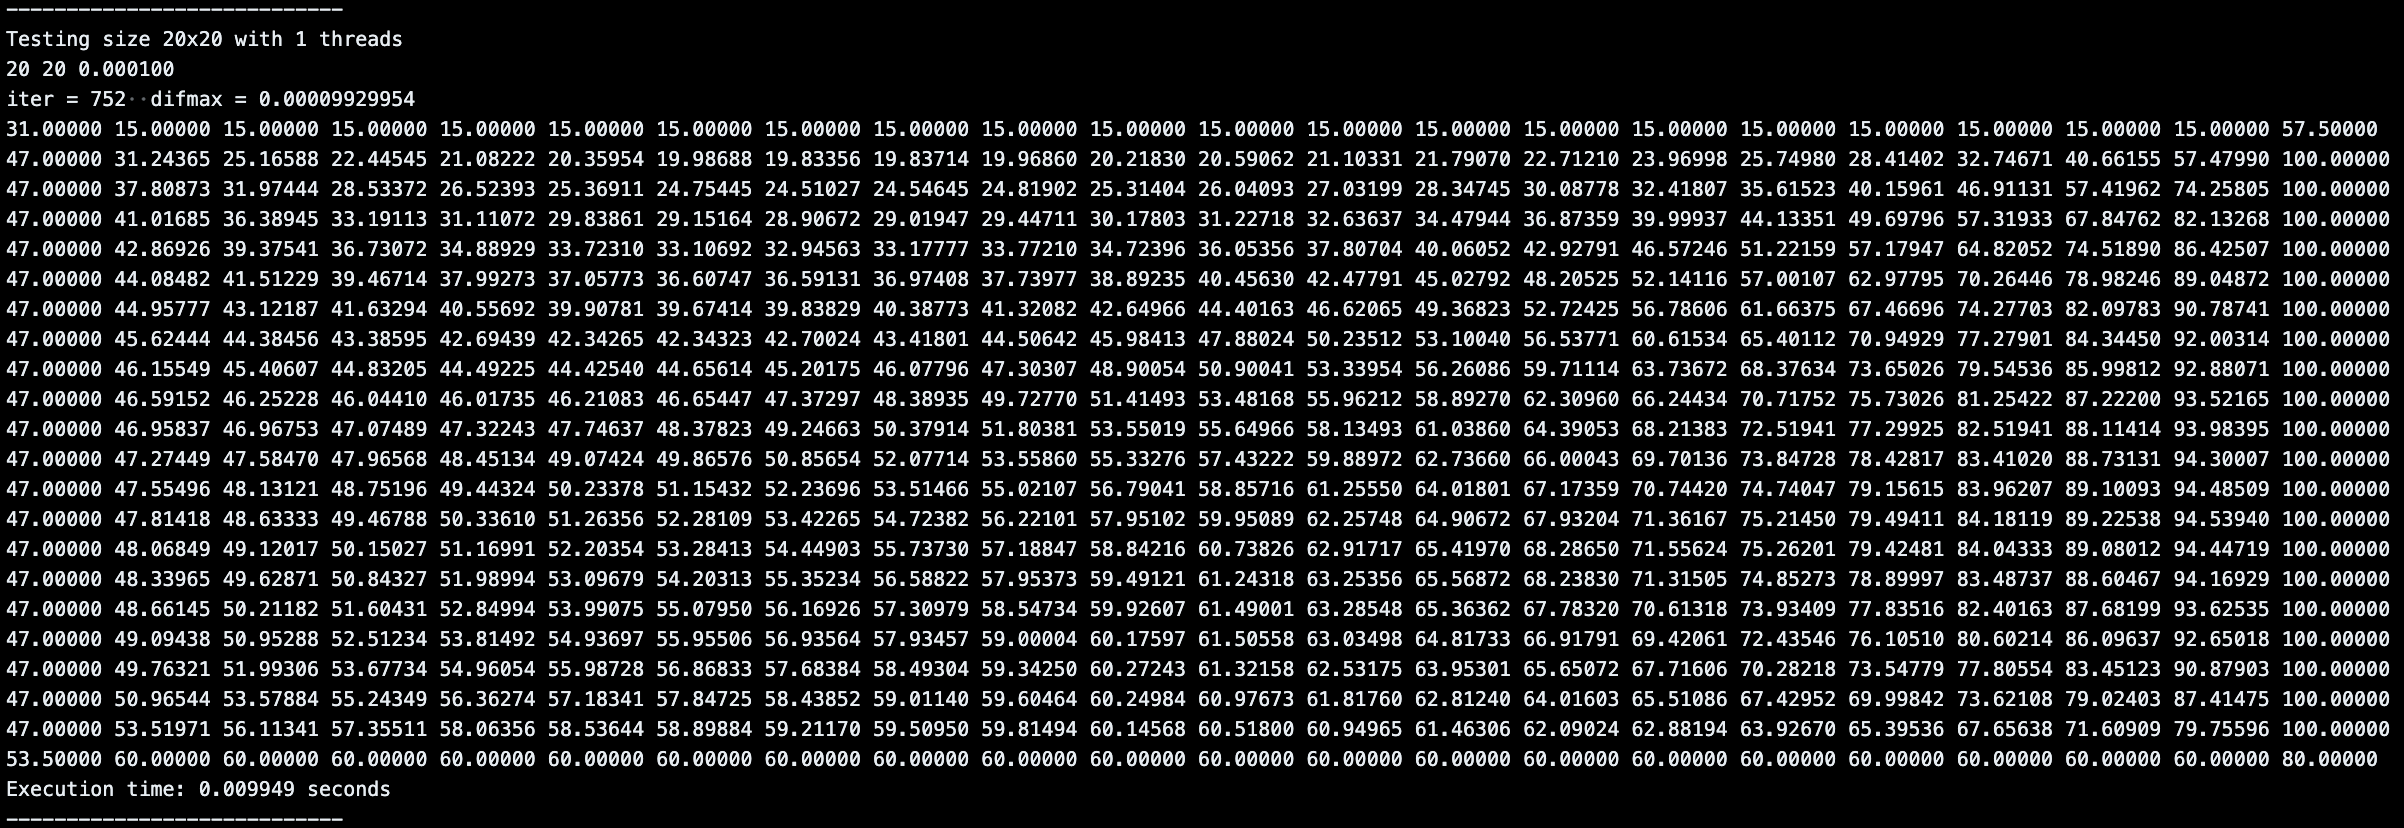
\includegraphics[width=\linewidth]{Images/Thread1.png}
    \caption{Screenshot of Thread Count 1}
    \label{fig:thread1}
\end{figure}

\begin{figure}[H]
    \centering
    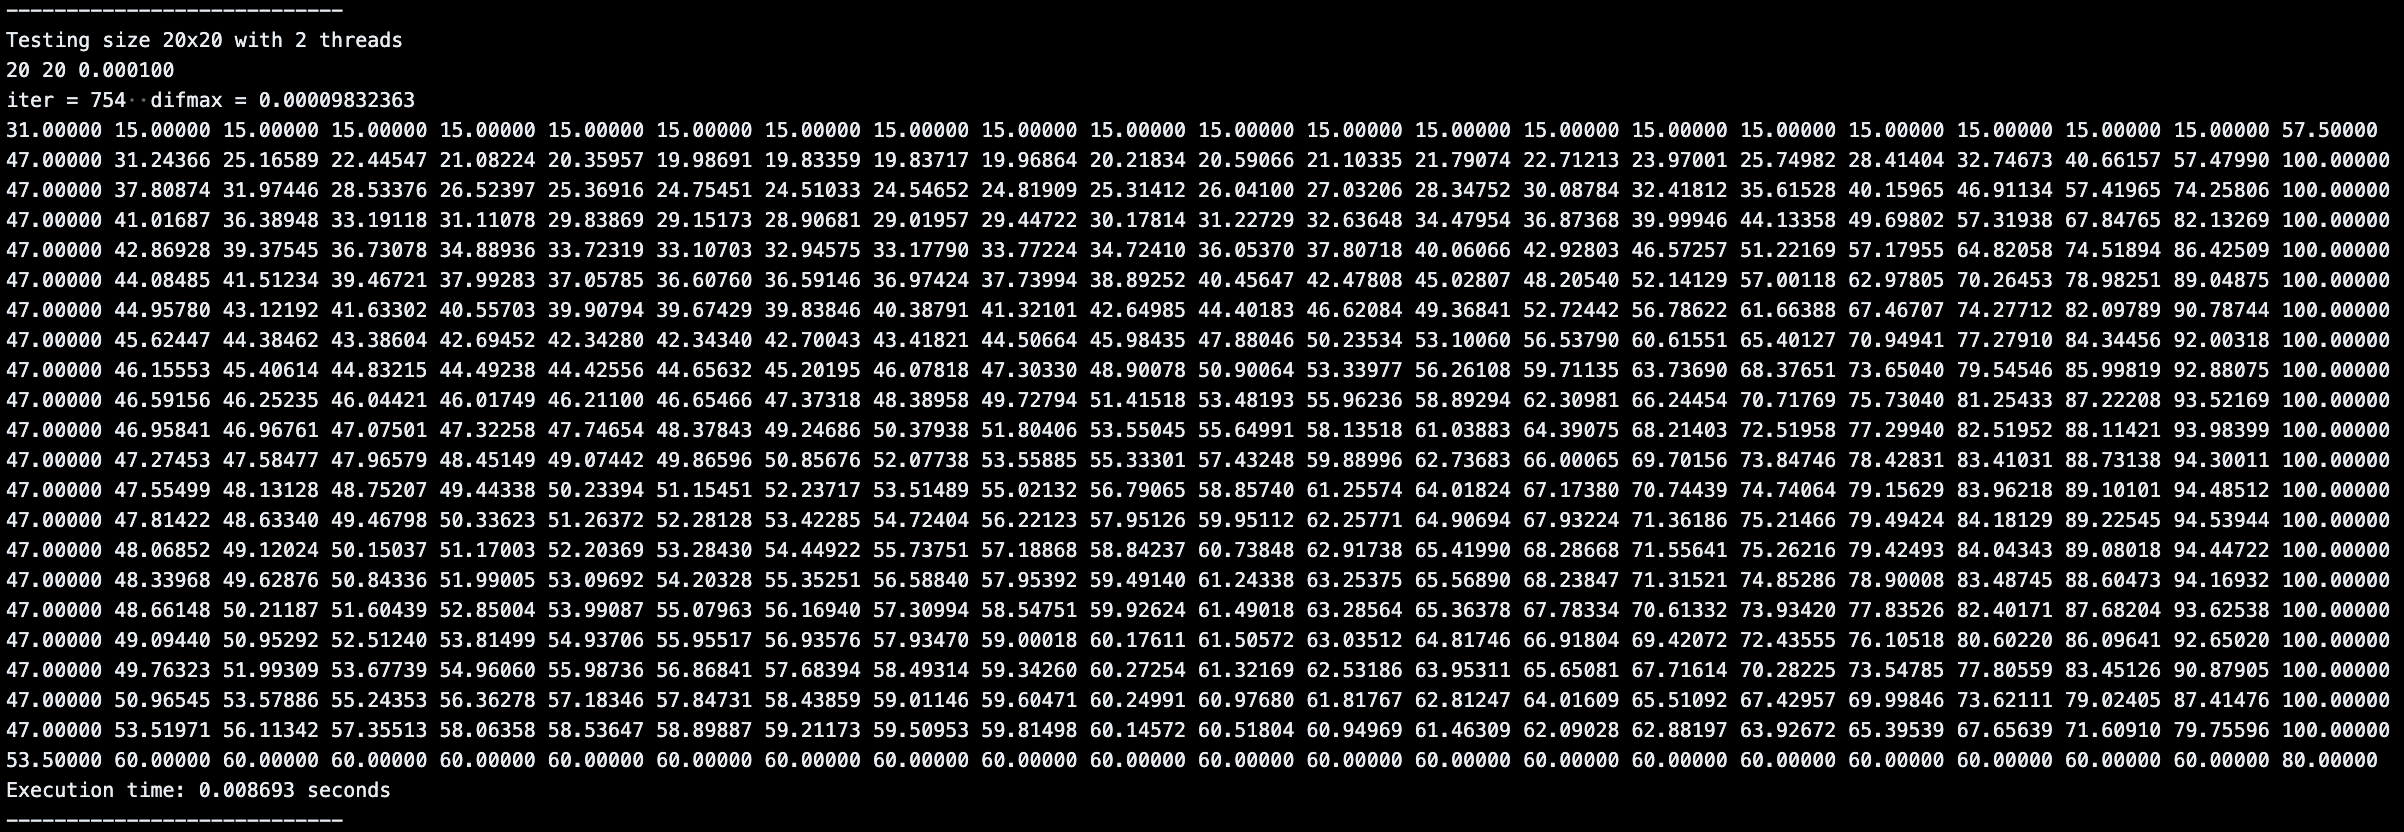
\includegraphics[width=\linewidth]{Images/Thread2.png}
    \caption{Screenshot of Thread Count 2}
    \label{fig:thread2}
\end{figure}

\begin{figure}[H]
    \centering
    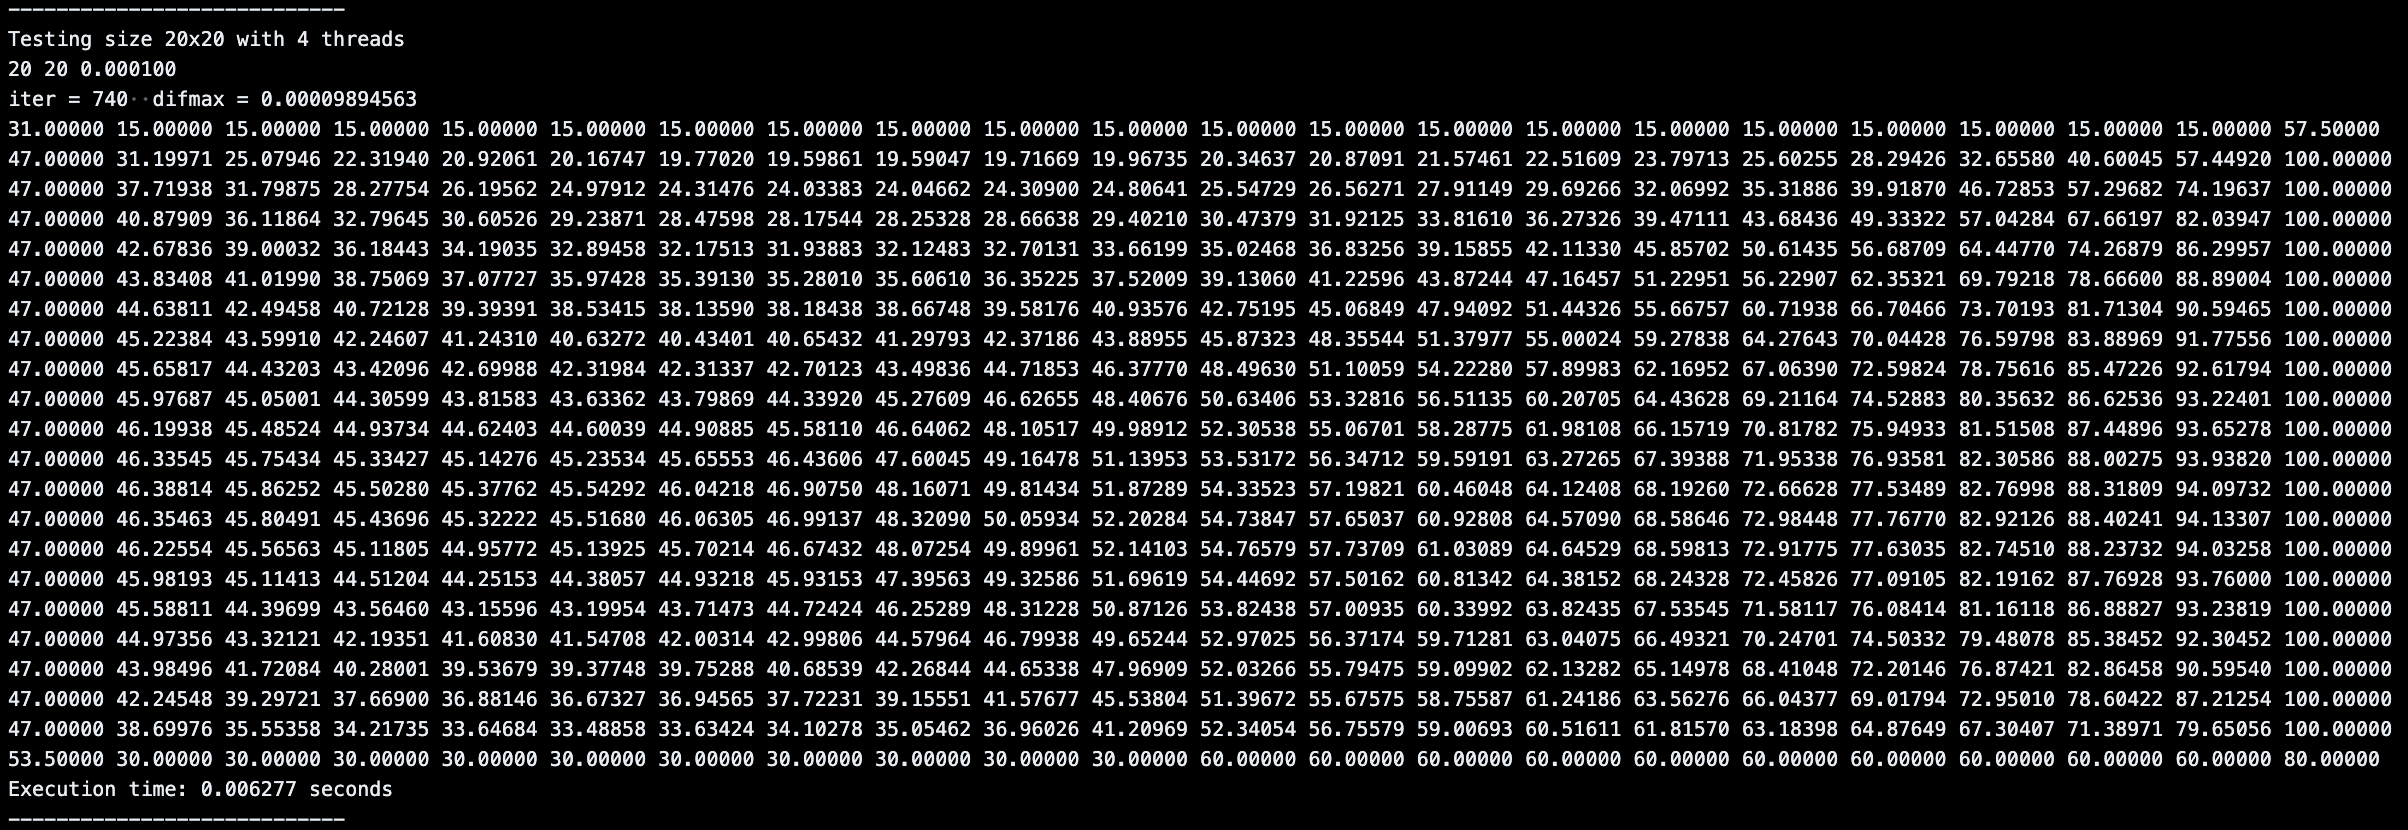
\includegraphics[width=\linewidth]{Images/Thread4.png}
    \caption{Screenshot of Thread Count 4}
    \label{fig:thread4}
\end{figure}

\begin{figure}[H]
    \centering
    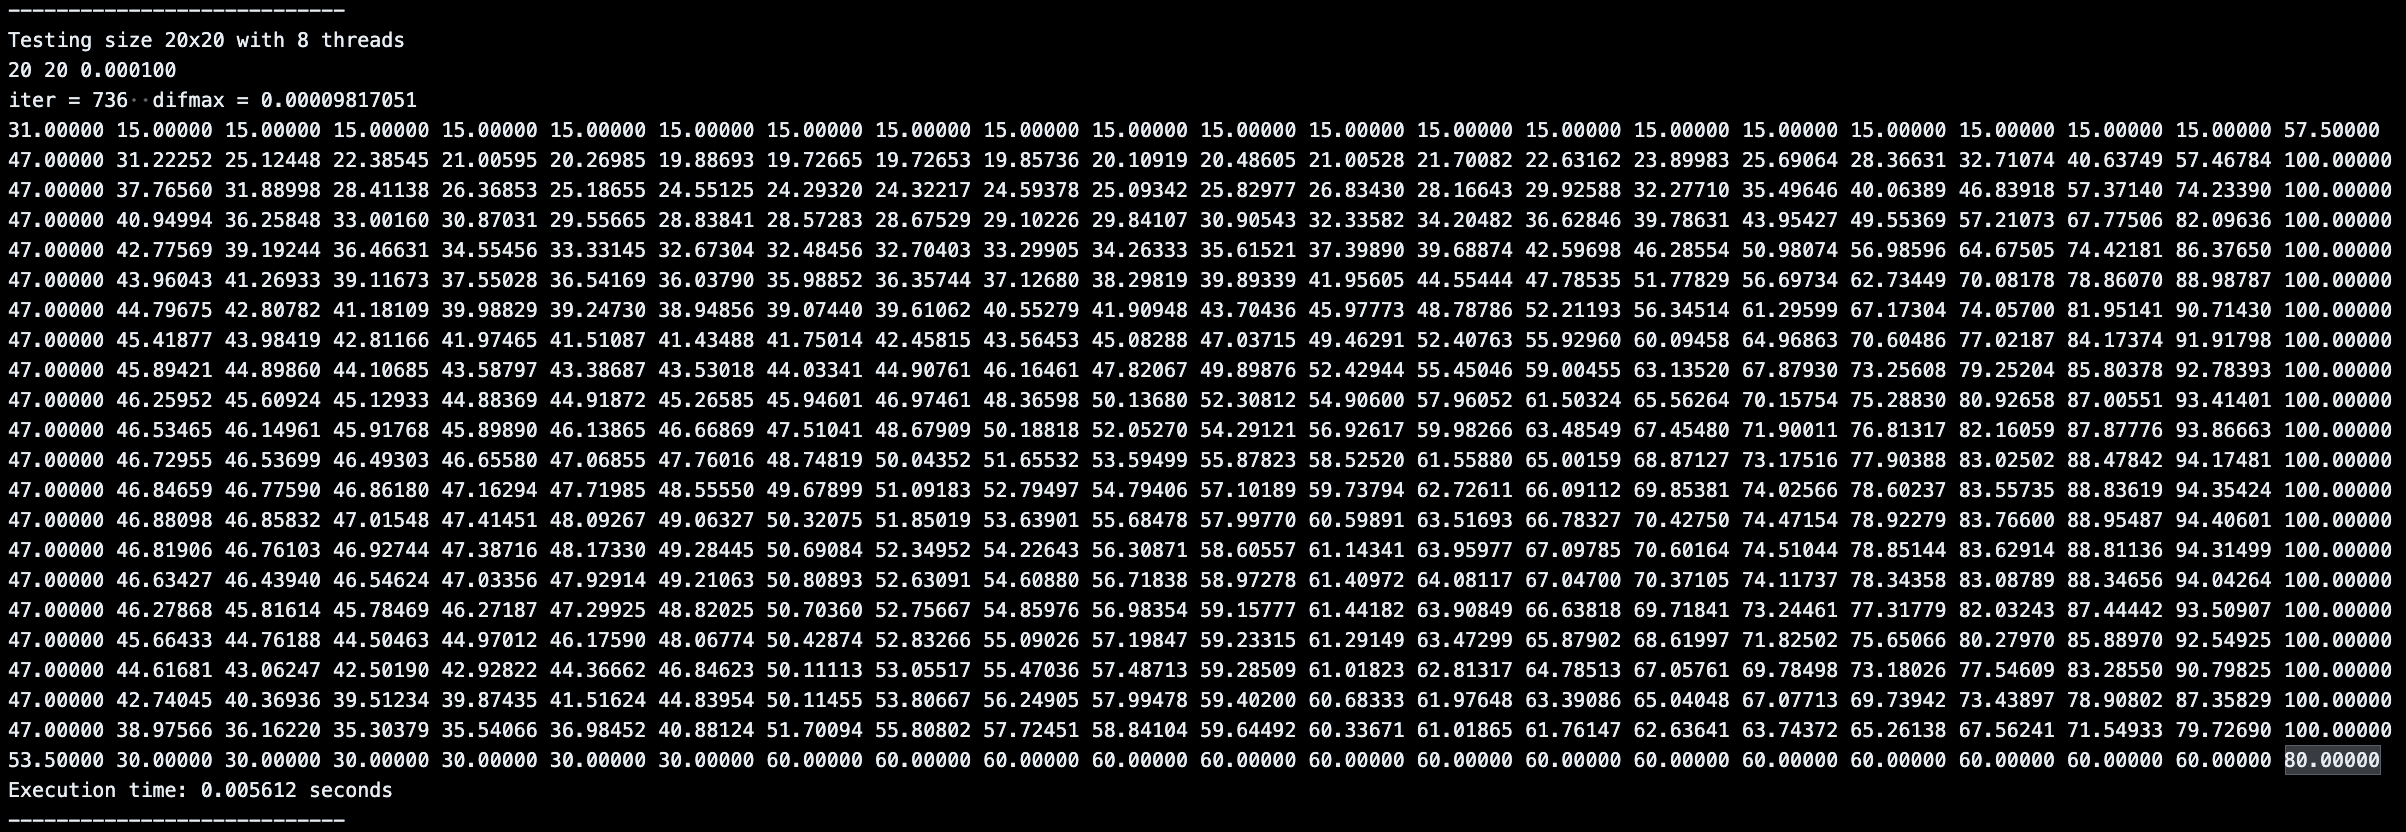
\includegraphics[width=\linewidth]{Images/Thread8.png}
    \caption{Screenshot of Thread Count 8}
    \label{fig:thread8}
\end{figure}

This outputs confirm that the temperature distribution conforms to the specified boundary conditions, and the program functions correctly for different thread counts.

\subsubsection{Recommendations for Further Work}

\begin{itemize}
    \item \textbf{Larger Problem Sizes:} Testing with larger grids would provide more insight into the scalability and efficiency of the parallel implementation.
    \item \textbf{Optimization Strategies:} Exploring different scheduling strategies and optimizing memory access patterns could further improve performance.
    \item \textbf{Hardware Considerations:} Running the program on hardware with more cores or different architectures may yield different performance characteristics.
\end{itemize}

\subsubsection{Conclusion}

The OpenMP parallelization of the Jacobi 2D grid problem successfully leveraged multiple threads to reduce execution time while maintaining correct results. The modifications to the code focused on parallelizing the initialization and main computation loops, utilizing OpenMP directives and clauses to manage data dependencies and reductions. The automated testing script facilitated consistent performance measurements across different thread counts, and the results demonstrate both the correctness and scalability of the parallel implementation.

\subsection{Step 3}



\printbibliography

\textit{Due to space constraints, only relevant portions of the code have been included in the main report. The full code is provided in the attached files.}

\end{document}